\chapter{Uvod}

Pojavom popularnih internetskih usluga za povezivanje korisnika stvorene su velike mreže društvenih zajednica. Generirane su velike količine podataka iz kojih je moguće izvući mnoštvo korisnih informacija. Takve zajednice sastoje se od puno manjih zajednica koje se po svojim karakteristikama razlikuju od ostalih. Zajednice je potrebno pronaći kako bi im se pristupilo na najbolji mogući način. Rješavanje ovog problema važno je i u drugim granama znanosti, kao na primjer u sociologiji, biologiji ili računarskoj znanosti, gdje su problemi predstavljeni na takav način, pomoću strukture grafa. 

Upravo su grafovi najpogodnija struktura podataka za pristup ovome problemu, gdje relevantne značajke, u primjeru društvenih mreža, ljude možemo prikazati pomoću čvorova, dok će bridovi predstavljati veze između tih značajki. Više bridova među određenim značajkama značit će da tu mogu postojati obilježja zajednice, npr. u biologiji bi to mogla biti tkiva koja u organima obavljaju sličnu ulogu. 

Rješavanje problema koji su predstavljeni grafovima je vrlo složeno, vremenski i prostorno. Ovakvi grafovi nisu jednostavnog oblika, ali u njima postoje određene pravilnosti, koje se mogu iskoristiti. U tu svrhu razvijeno je mnogo algoritama za otkrivanje zajednica koji različitim pristupima pokušavaju pronaći rješenje ovog problema. Pojedini algoritmi su bolji od drugih na jednom tipu društvenih mreža ili lošiji na drugom te se zato koriste evaluacijske mjere kojima se procjenjuje koliko je dobro rješenje koje je algoritam pronašao. Što više algoritama se testira s različitim društvenim mrežama i evaluacijskim mjerama dobit će se bolji uvid u to kada je koji bolje koristiti. Najpoznatiji algoritam među njima je Girvan-Newmanov algoritam koji će se nešto detaljnije opisati uz još nekoliko njih. Sličnim problemima bavili su se radovi Lancichinettija i Fortunata \cite{fortunato2016community} iz 2016. te \cite{lancichinetti2009community} iz 2009. godine.

Unatrag nekoliko posljednjih  godina uvedeni su zakoni o zaštiti osobnih podataka te je sada znatno teže dobiti pristup korisnim informacijama. Zato se koriste posebni algoritmi za generiranje umjetnih skupova podataka koji će za zadane parametre generirati grafovi pomoću kojih se mogu provoditi istraživanja. Kako bi generirani grafovi bili iskoristivi moraju zadovoljavati svojstva karakteristična grafovima društvenih mreža koja se očituju u kratkoj udaljenosti između bilo koja dva čvora grafa te u visokom koeficijentu grupiranja. Mreže koje imaju navedena svojstva nazivaju se small-world mreže.

U nastavku rada bit će opisana struktura i svojstva društvenih mreža i zajednica, algoritmi koji pronalaze društvene zajednice, skupovi podataka koji su korišteni u sklopu rada, programsko rješenje koje pokreće i evaluira rješenja algoritama te će se prikazati i rezultati  do kojih se došlo. 


\begin{figure}
	\makebox[\textwidth][c]{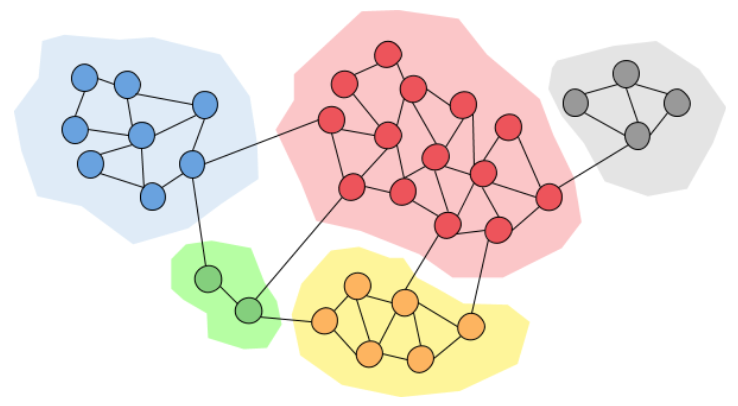
\includegraphics[width=0.8\textwidth]{images/simple-community.png}}
	\caption{Primjer grafa nepreklapajućih društvenih zajednica \cite{jayawickrama_2021}.}
	\label{fig:comm1}
\end{figure}
